% History
% 12/06/2024  (岸)	修論下書き用texファイル作成
% 12/12/2024  (岸)	フォントサイズを11pt, 行間を1.5に設定
% コンパイルの仕方
% 		uplatex chapter1_v1.tex
% 		pbibtex chapter1_v1
% 		uplatex chapter1_v1.tex
% 		uplatex chapter1_v1.tex
% 		dvipdfmx chapter1_v1.dvi

% フォントサイズを11ptに設定
\documentclass[a4paper,11pt,nomag]{jsreport}

\usepackage[dvipdfm,truedimen]{geometry}
\geometry{top=22mm,bottom=22mm,left=22mm,right=22mm}

%\usepackage{layout}
%\usepackage[utf8]{inputenc} %不要かも
\usepackage[T1]{fontenc} %utf8フォントエンコーディング指定
\usepackage{lmodern} % 11pt, nomag を使っているので
\usepackage{array}
\newcommand{\bhline}[1]{\noalign{\hrule height #1}}  
\newcommand{\bvline}[1]{\vrule width #1}
\renewcommand{\baselinestretch}{1.5} % 教授が赤修正を入れやすいように行間を1.5に設定
\usepackage[subrefformat=parens]{subcaption}
\usepackage[dvipdfmx]{graphicx} % dvipdfmx を前提としている
\usepackage[dvipdfmx]{color}
\usepackage{caption}
\usepackage{subcaption}
\usepackage{bbm}
\usepackage{multirow}
\usepackage{arydshln}
\usepackage{here} % 図表の位置決め用
\usepackage{amsmath,amssymb}% 数式用
\usepackage{url}      % URL等記載用.\verbより便利
\usepackage{enumerate}
\usepackage{midpage}

% サブキャプションのフォーマットを調整
\renewcommand\thesubfigure{(\alph{subfigure})}
\captionsetup[subfigure]{labelformat=simple, labelsep=space}

\begin{document}

\chapter*{序論}

生物多様性が生み出す生態的機能は,温室効果ガス,エネルギー,水などの物質・資源循環など,地球に不可欠な役割を多数持っており,人間社会の基盤となっている \cite{millennium-ecosystem2005,cardinale2011}.
生態的機能のうち,特に人間社会の便益につながるものを生態系サービスと呼ぶ.
しかしながら,昨今,人間による土地開発や気候変動によって,陸域生態系の劣化と生物多様性の損失は進行しており \cite{newbold2015,isbell2017},生態系サービスの享受が困難になっている.
したがって,生態系の劣化を低減し,生物多様性の損失を抑制することは,現代社会における根本的な社会課題であり,その解決が急務である.
これらの課題は持続可能な開発目標(SDG15: 陸の豊かさも守ろう)などの国際目標としても掲げられ,日本でも生物多様性国家戦略 \cite{biodiversity2023}をはじめとする様々な政策や企業の取り組みが開始されている.

これらの社会課題に対して,継続的な野生動物との共存を実現するため,生態系モニタリングが注目を集めている.
生態系モニタリングは,自然環境の空間的・時間的変化の把握に有効な方法であり,自然保護や環境保全に重要なデータを提供する.
モニタリング実施の効果として生態系に生じた異常の早期発見が可能であり,迅速な対策により生態系の回復期間の短縮やコスト削減へと繋がることが期待される.

費用対効果の高い生態系モニタリングを行う上で,カメラトラップの使用は極めて重要である \cite{jia2022}.
カメラトラップは,赤外線センサなどを用いてカメラの前を通り過ぎる動物を感知し,自動的に撮影するため,動物にストレスを与えることなく,撮影者によるバイアスを排除したデータ収集が可能である\cite{newey2015,zhu2017}.
これらのカメラは,比較的低価格であり,限られた電力資源で効率的に動作するため,広範囲に長期間の撮影が可能である \cite{schneider2018, carl2020}.
また,赤外線カメラの使用により,夜間の撮影も可能である.
近年,カメラトラップによって膨大な画像や動画データが低コストで収集できるようになり,深層学習モデルを用いた野生動物の正確な検出と分類に期待が高まっている \cite{tan2022}.

野生動物画像の分類に関して,畳み込みニューラルネットワーク (Convolutional Neural Network,CNN) を用いた手法がいくつか提案されている \cite{manna2023,mohanty2022, agarwal2023, neeli2023}.
しかし,自然環境下における野生動物に対する分類タスク特有の課題として,特定地域における十分な量の学習用画像の収集コストが高いことや \cite{schneider2020},赤外線カメラによって撮影された画像は色情報が欠落していること \cite{kishimoto2023}などが挙げられる.
図 \ref{fig:camera}に撮影方法(カメラ)の違いによる物体の写り方の違いを示す.
既存の動物分類手法のほとんどは図 \ref{fig:color_deer}のような可視光画像に焦点を当てており,図\ref{fig:infrared_deer}のような赤外線画像に対して取り組んだ研究は少ない.
また,赤外線画像と可視光画像では物体の写り方が大きく異なるため,既存の可視光画像に対する手法を赤外線画像に対して適用した場合,精度が大きく低下する.

\begin{figure}[tbp]
  \centering
  \begin{subfigure}[b]{0.45\linewidth}
    \centering
    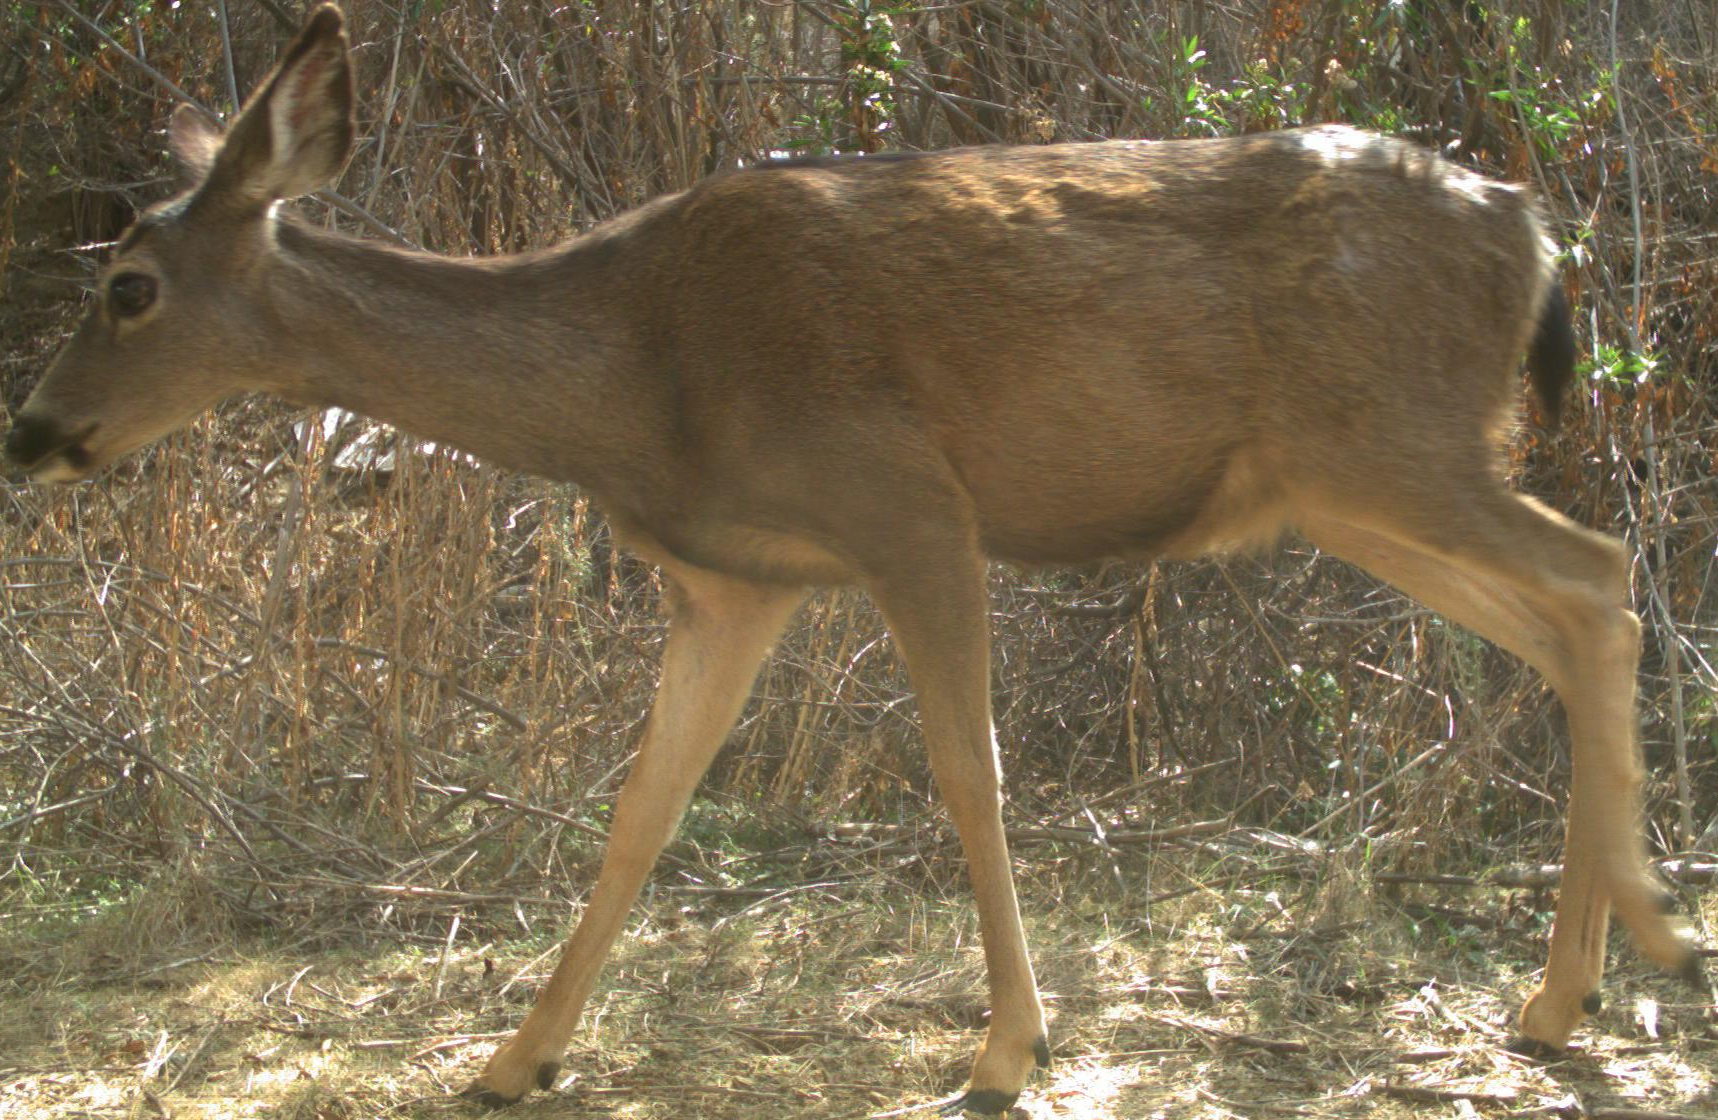
\includegraphics[height=0.7\linewidth, keepaspectratio]{cct_color_deer.png}
    \caption{可視光画像}
    \label{fig:color_deer}
  \end{subfigure}
  \hfill
  \begin{subfigure}[b]{0.45\linewidth}
    \centering
    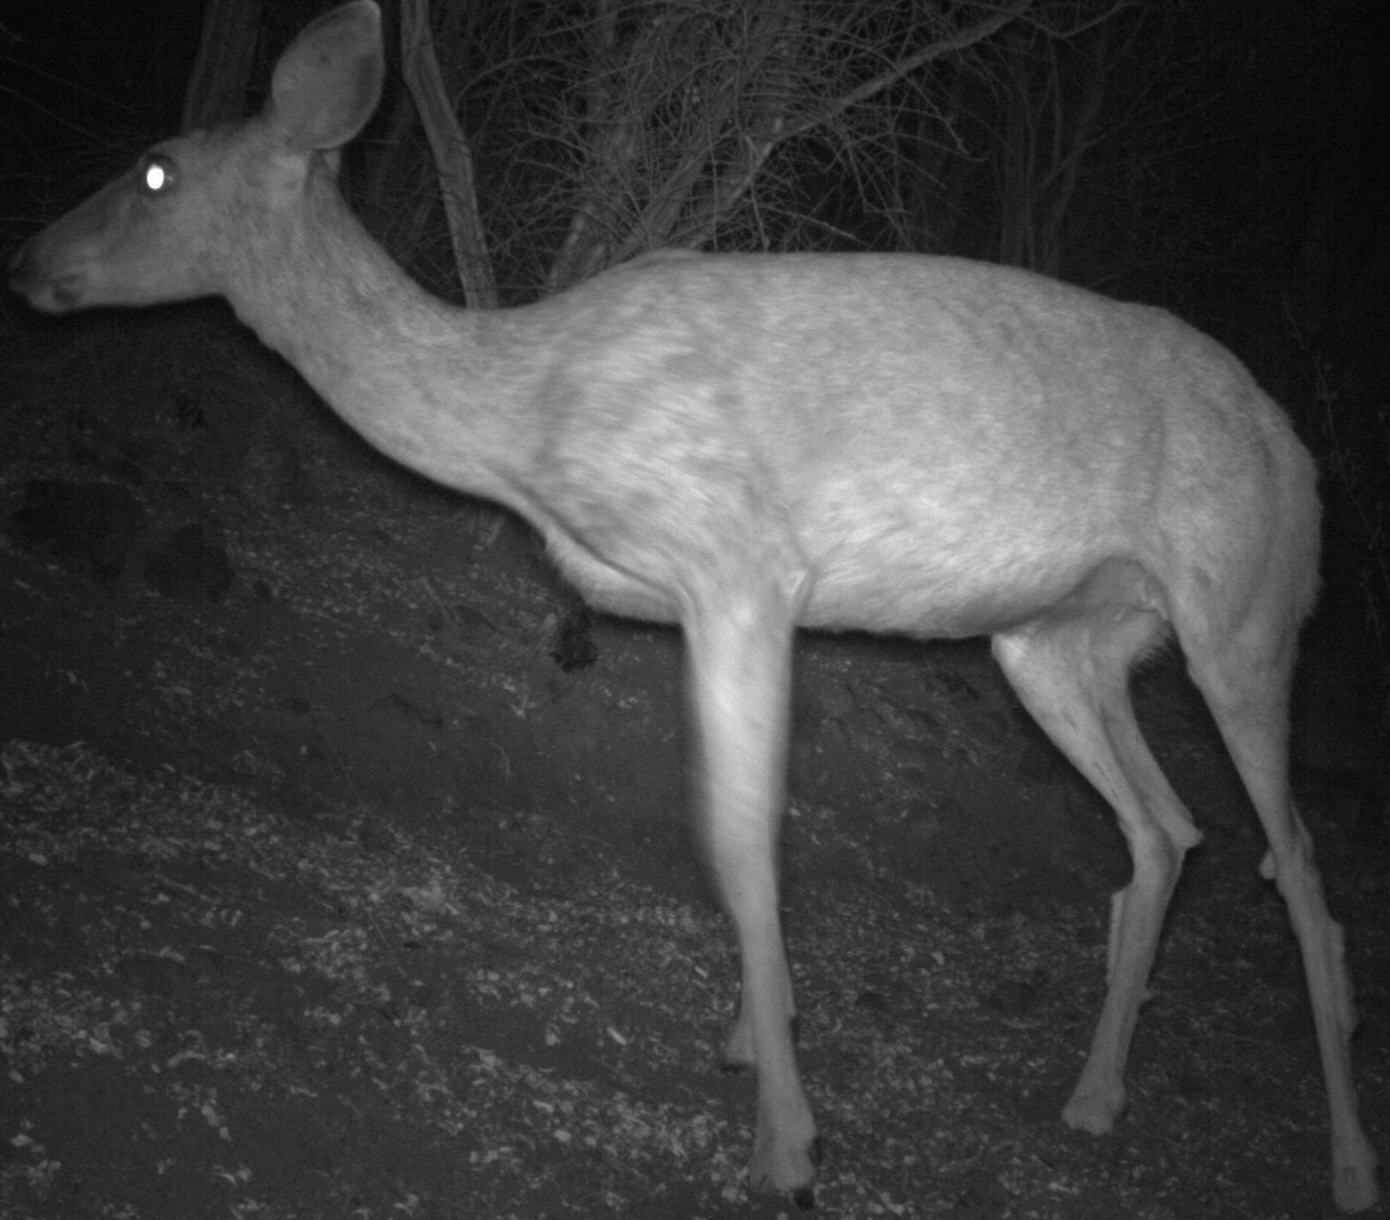
\includegraphics[height=0.7\linewidth, keepaspectratio]{cct_infrared_deer.png}
    \caption{赤外線画像}
    \label{fig:infrared_deer}
  \end{subfigure}
  \caption{撮影方法(カメラ)の違いによる物体の写り方}
  \label{fig:camera}
\end{figure}

このような課題を解決するため,少数の赤外線画像を深層学習モデルの学習に用いた動物分類に関する研究が行われている \cite{kishimoto2023}.
しかし,既存研究では,評価時に分類対象となる動物種は全て学習済みであると仮定しているが,実運用において,深層学習モデルを特定の地域に適用する際,モデルが対象地域に生息する全ての動物種を学習しているとは限らない.
このような状況において,未学習の動物種は学習済みの動物種に強制的に誤分類され,モデルの性能は著しく低下することが知られており,この問題はオープンセット問題 (Open-Set Problem) と呼ばれる.
オープンセット問題に対処するため,学習済みクラスの分類を行いつつ,未学習クラスを検出するオープンセット認識 (Open-Set Recognition,OSR) 手法が提案されている \cite{sun2020, sagar2022}.

さらに近年では,少数データでもオープンセット認識を可能にする Few-Shot Open-Set Recognition (FSOSR) \cite{peeler} が注目を集めている.
代表的なFSOSR手法として,少数データ学習 (Few-Shot Learning,FSL) 分野で有効な手法とされているメタ学習をOSRに拡張することによりFSLとOSRを同時に実現したPEELER \cite{peeler}や,変換の一貫性に基づき未学習クラスを検出することによって,擬似的な未学習クラスサンプルを必要としないSnaTCHer \cite{snatcher}が挙げられる.
しかし,これらの手法は可視光画像を対象としており,赤外線画像に対して性能評価がなされていない.
また,FSOSRでは未学習クラスを単一種として扱っているが,未学習クラスのアノテーションや追加学習を考慮すると,実用的には未学習クラスも複数種に分類できることが望ましい.

本論文では,夜間の野生動物モニタリングの実現を目的とした,より実用的な問題設定である「Infrared Few-shot Open-set Recognition (IFOR)」を提案する.
IFORでは少量の赤外線画像データのみを用いて,特定地域に生息するモデルに学習済みの動物種を正確に分類し,かつ,未学習の動物種の検出を可能にすることを目指す.
加えて,IFORではドメインシフトに対する頑健性の評価も必要である.
ドメインシフトとは,学習データと評価データが異なる地域で収集された場合に生じる課題であり,背景や撮影環境の違い,同じ動物種の地域差による外見の違いによってモデルの性能が低下する現象を指す.
ドメインシフトを考慮することにより,地理的条件に依存せず,様々な場所に適用可能な汎用性の高いシステムの実現が期待される.

本論文では,IFORの実現に向けて,赤外線画像に有効な既存手法の特定に加え,既存のFSOSR手法の1つであるメタ学習フレームワークがIFORに対して効果的であるか検証を行う.
まず,赤外線画像に有効な特徴抽出器を特定するため,テクスチャ特徴に焦点を当てているCNNや,形状特徴 \cite{feature}を重視することで知られている Vision Transformer (ViT) \cite{vit}などの代表的な特徴抽出器の有効性を赤外線画像に対して評価する.
次に,IFORフレームワーク内のFSLタスクに有効なアプローチの1つである転移学習について検証する.
転移学習では,事前学習のタスクと本番環境でのタスクの類似度が重要だと考えられている.
そこで,一般的なImageNetデータセットを用いた事前学習と並行して,事前学習に色情報を持たないフラクタル画像を用いるFormula-Driven Supervised Learning (FDSL) \cite{fdsl}の有効性を探る.
最後に,赤外線画像を分類する際,小規模データセットから汎用的な特徴抽出を行うための学習戦略であるメタ学習のIFORにおける有効性を,ドメインシフトの条件下で評価する.
特に,IFORにおいては学習済みクラスの正確な画像分類と未学習クラスの検出が不可欠であるため,メタ学習による有効性を従来の学習方法であるミニバッチ学習と比較する.

さらに,IFORを発展させ,未学習クラスに対する多クラス分類の精度向上にも取り組む.
特徴空間上で各学習済みクラスの分布がコンパクトに表現されることにより,未学習データに対しても多クラス分類が容易になると仮定し,クラスタリンに基づく損失関数を用いてクラス内分散の最小化・クラス間分散の最大化を図る.
クラス内分散の最小化では,異常検知タスクで用いられているk-means損失 \cite{k-means} を導入する.
クラス間分散の最大化では,k-meansクラスタリングによって得られる各クラスタ中心を利用した損失関数であるBetween-Class損失 (BC損失) を提案する.

以下,第2章では深層学習を用いた動物分類に関する既存研究について述べる.
第3章では夜間の野生動物モニタリングの実現に向けてより実用的な問題設定を提案し,様々な手法の有用性について述べる.
第4章では評価実験を行い,その結果及び考察を多面的な方向性から述べる.
最後に第5章では結論を述べる.

% ここから参考文献bibtexの設定
\bibliographystyle{kishiIEEEtr}
\bibliography{references}

\end{document}